%
%  Contains the appendix for the thesis
%
% For a single appendix, use \makeappendix, and place the
% body of the appendix after it

%\makeappendix

% < single appendix body here >

% For multiple appendices, use \makeappendices, and create each appendix
% using \appendix{}
% For sub-appendices use \appendixsection{} and \appendixsubsection{}

\makeappendices
\appendix{Voting Distributions}\label{chap:voting-distributions}

\appendixsection{Percent inside Extents}
\autoref{tab:distributions-percent-inside-extents} displays the percent of votes that
remain inside the desired extents per distribution.

\begin{table}[htbp]
    % increase table row spacing, adjust to taste
    \renewcommand{\arraystretch}{1.3}

    \caption{The percent of votes that remain inside the desired extents.}
    \label{tab:distributions-percent-inside-extents}

    \centering
    \begin{tabular}{|c|c|c|}
        \hline
        Distribution      & Notation      & Percent inside Extents \\
        \hhline{|=|=|=|}
        Uniform           & \uniformdist  & 100\%                  \\
        \hline
        Normal (Gaussian) & \gaussiandist & 99.7\%                 \\
        \hline
        Beta              & \betadist     & 100\%                  \\
        \hline
    \end{tabular}
\end{table}

\appendixsection{Distributions used}
The following distributions are used by agents to vote:
\begin{itemize}
    \item Uniform (\uniform{-1}{1}; \autoref{fig:uniform})
    \item Gaussian (\gaussian{0}{\frac{1}{3}}; \autoref{fig:gaussian})
    \item Beta(0.3, 0.3) (\betadistribution{0.3}{0.3}; \autoref{fig:beta-0.3-0.3})
    \item Beta(0.3, 4) (\betadistribution{0.3}{3}; \autoref{fig:beta-0.3-3})
    \item Beta(3, 0.3) (\betadistribution{3}{0.3}; \autoref{fig:beta-3-0.3})
    \item Beta(4, 4) (\betadistribution{4}{4}; \autoref{fig:beta-4-4})
    \item Beta(1, 4) (\betadistribution{1}{4}; \autoref{fig:beta-1-4})
    \item Beta(4, 1) (\betadistribution{4}{1}; \autoref{fig:beta-4-1})
\end{itemize}

\begin{figure}[!h]
    \centering
    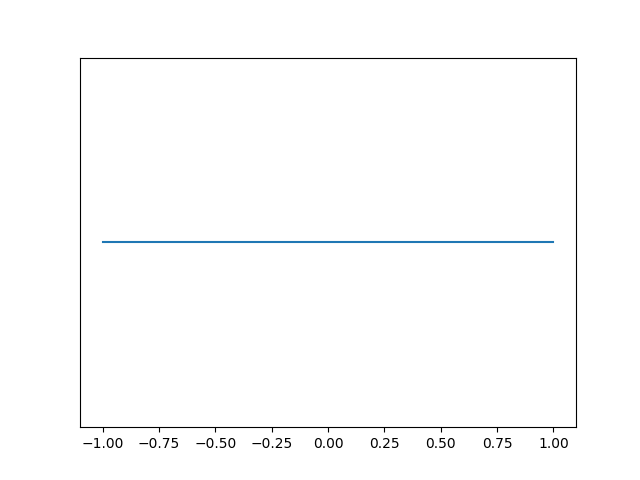
\includegraphics[scale=0.5]
    {./content/figures/dists/uniform}
    \caption{\uniform{-1}{1}}
    \label{fig:uniform}
\end{figure}

\begin{figure}[!h]
    \centering
    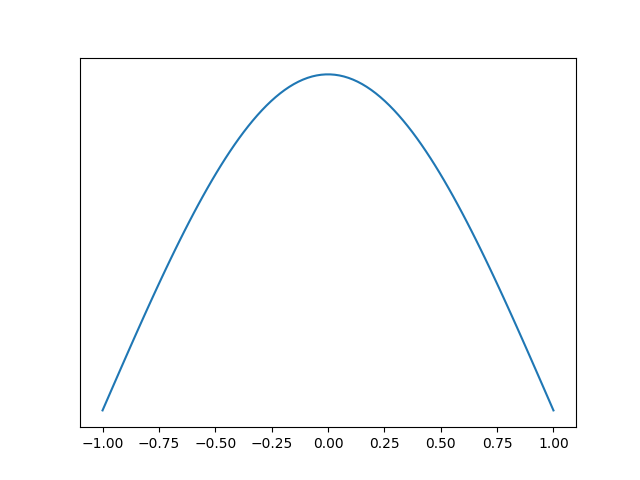
\includegraphics[scale=0.5]
    {./content/figures/dists/gaussian}
    \caption{\gaussian{0}{\frac{1}{3}}}
    \label{fig:gaussian}
\end{figure}

\begin{figure}[!h]
    \centering
    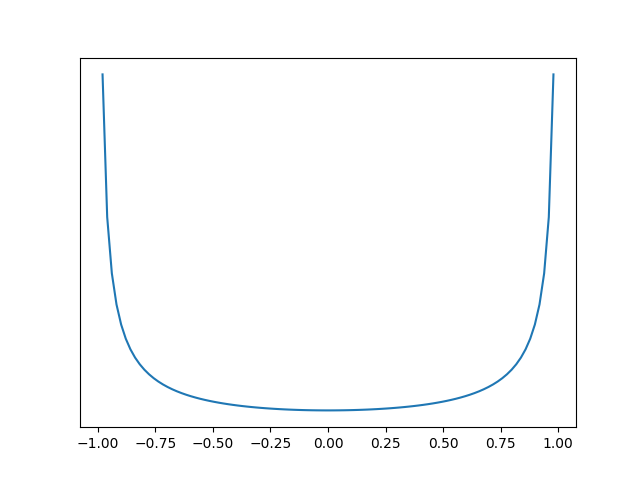
\includegraphics[scale=0.5]
    {./content/figures/dists/beta_0.3_0.3}
    \caption{\betadistribution{0.3}{0.3}}
    \label{fig:beta-0.3-0.3}
\end{figure}

\begin{figure}[!h]
    \centering
    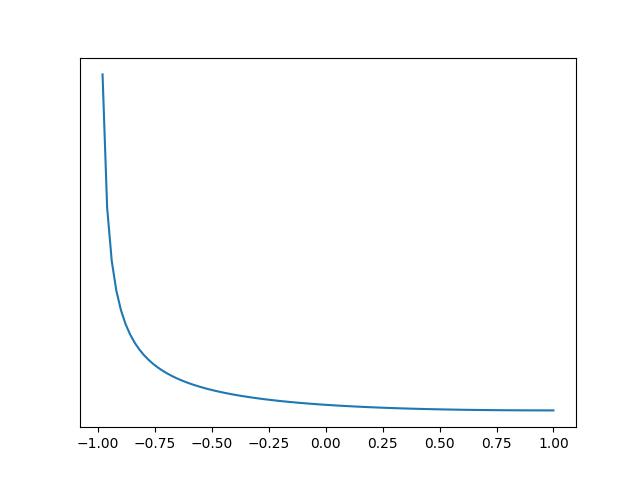
\includegraphics[scale=0.5]
    {./content/figures/dists/beta_0.3_3}
    \caption{\betadistribution{0.3}{3}}
    \label{fig:beta-0.3-3}
\end{figure}

\begin{figure}[!h]
    \centering
    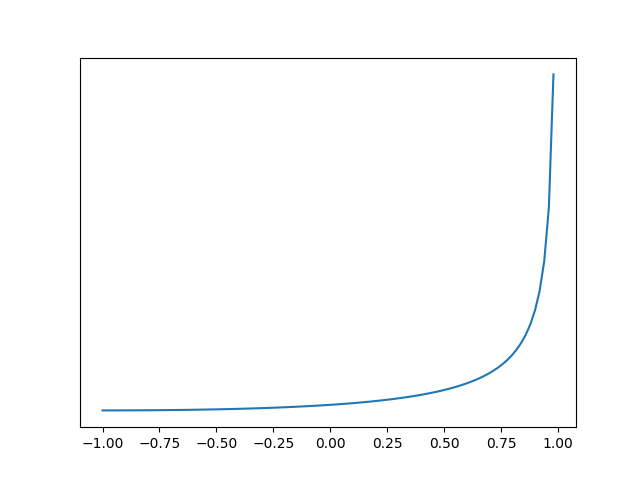
\includegraphics[scale=0.5]
    {./content/figures/dists/beta_3_0.3}
    \caption{\betadistribution{3}{0.3}}
    \label{fig:beta-3-0.3}
\end{figure}

\begin{figure}[!h]
    \centering
    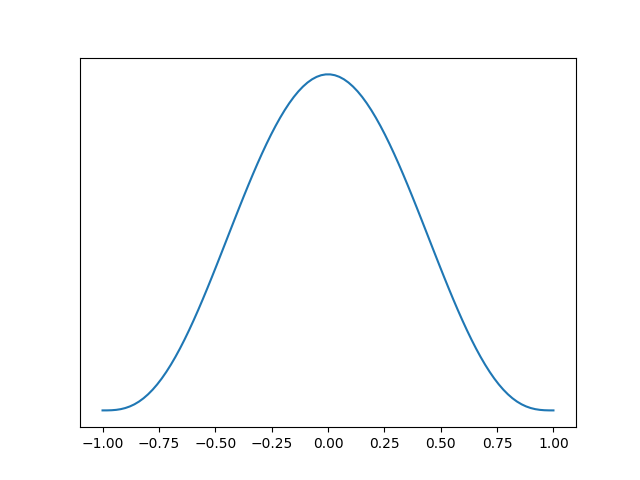
\includegraphics[scale=0.5]
    {./content/figures/dists/beta_4_4}
    \caption{\betadistribution{4}{4}}
    \label{fig:beta-4-4}
\end{figure}

\begin{figure}[!h]
    \centering
    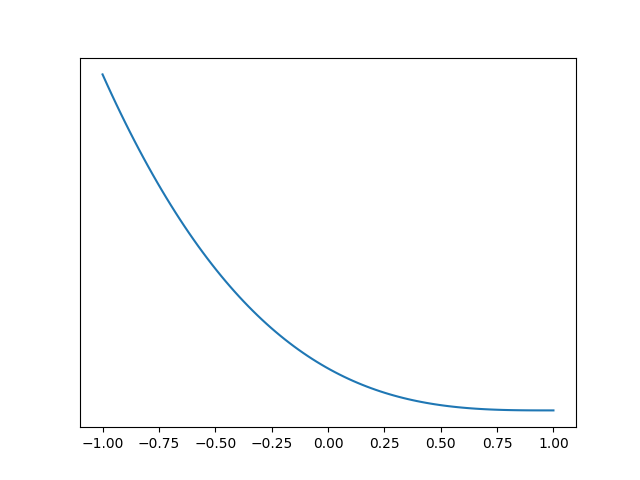
\includegraphics[scale=0.5]
    {./content/figures/dists/beta_1_4}
    \caption{\betadistribution{1}{4}}
    \label{fig:beta-1-4}
\end{figure}

\begin{figure}[!h]
    \centering
    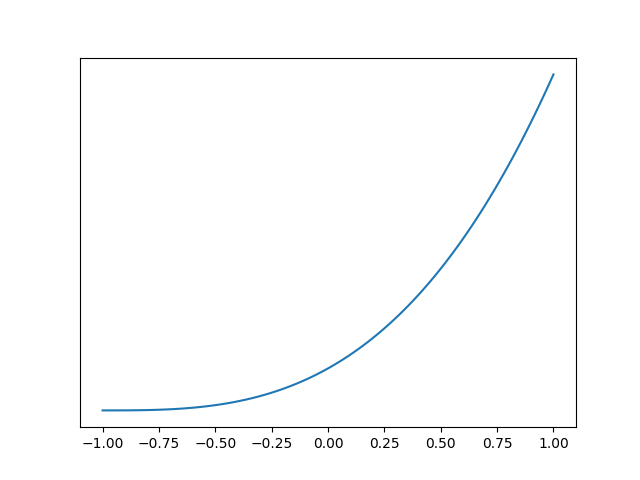
\includegraphics[scale=0.5]
    {./content/figures/dists/beta_4_1}
    \caption{\betadistribution{4}{1}}
    \label{fig:beta-4-1}
\end{figure}

\appendixsection{Voting Mechanism P-Values}
\autoref{fig:all-voting-mechanisms-p-values} illustrates the p-values for all voting
mechanisms, given the alternative is one population is lesser than the other.
An arrow pointing to another voting mechanism indicates the `from' mechanism beats
the `to' mechanism.

\begin{figure}[!t]
    \centering
    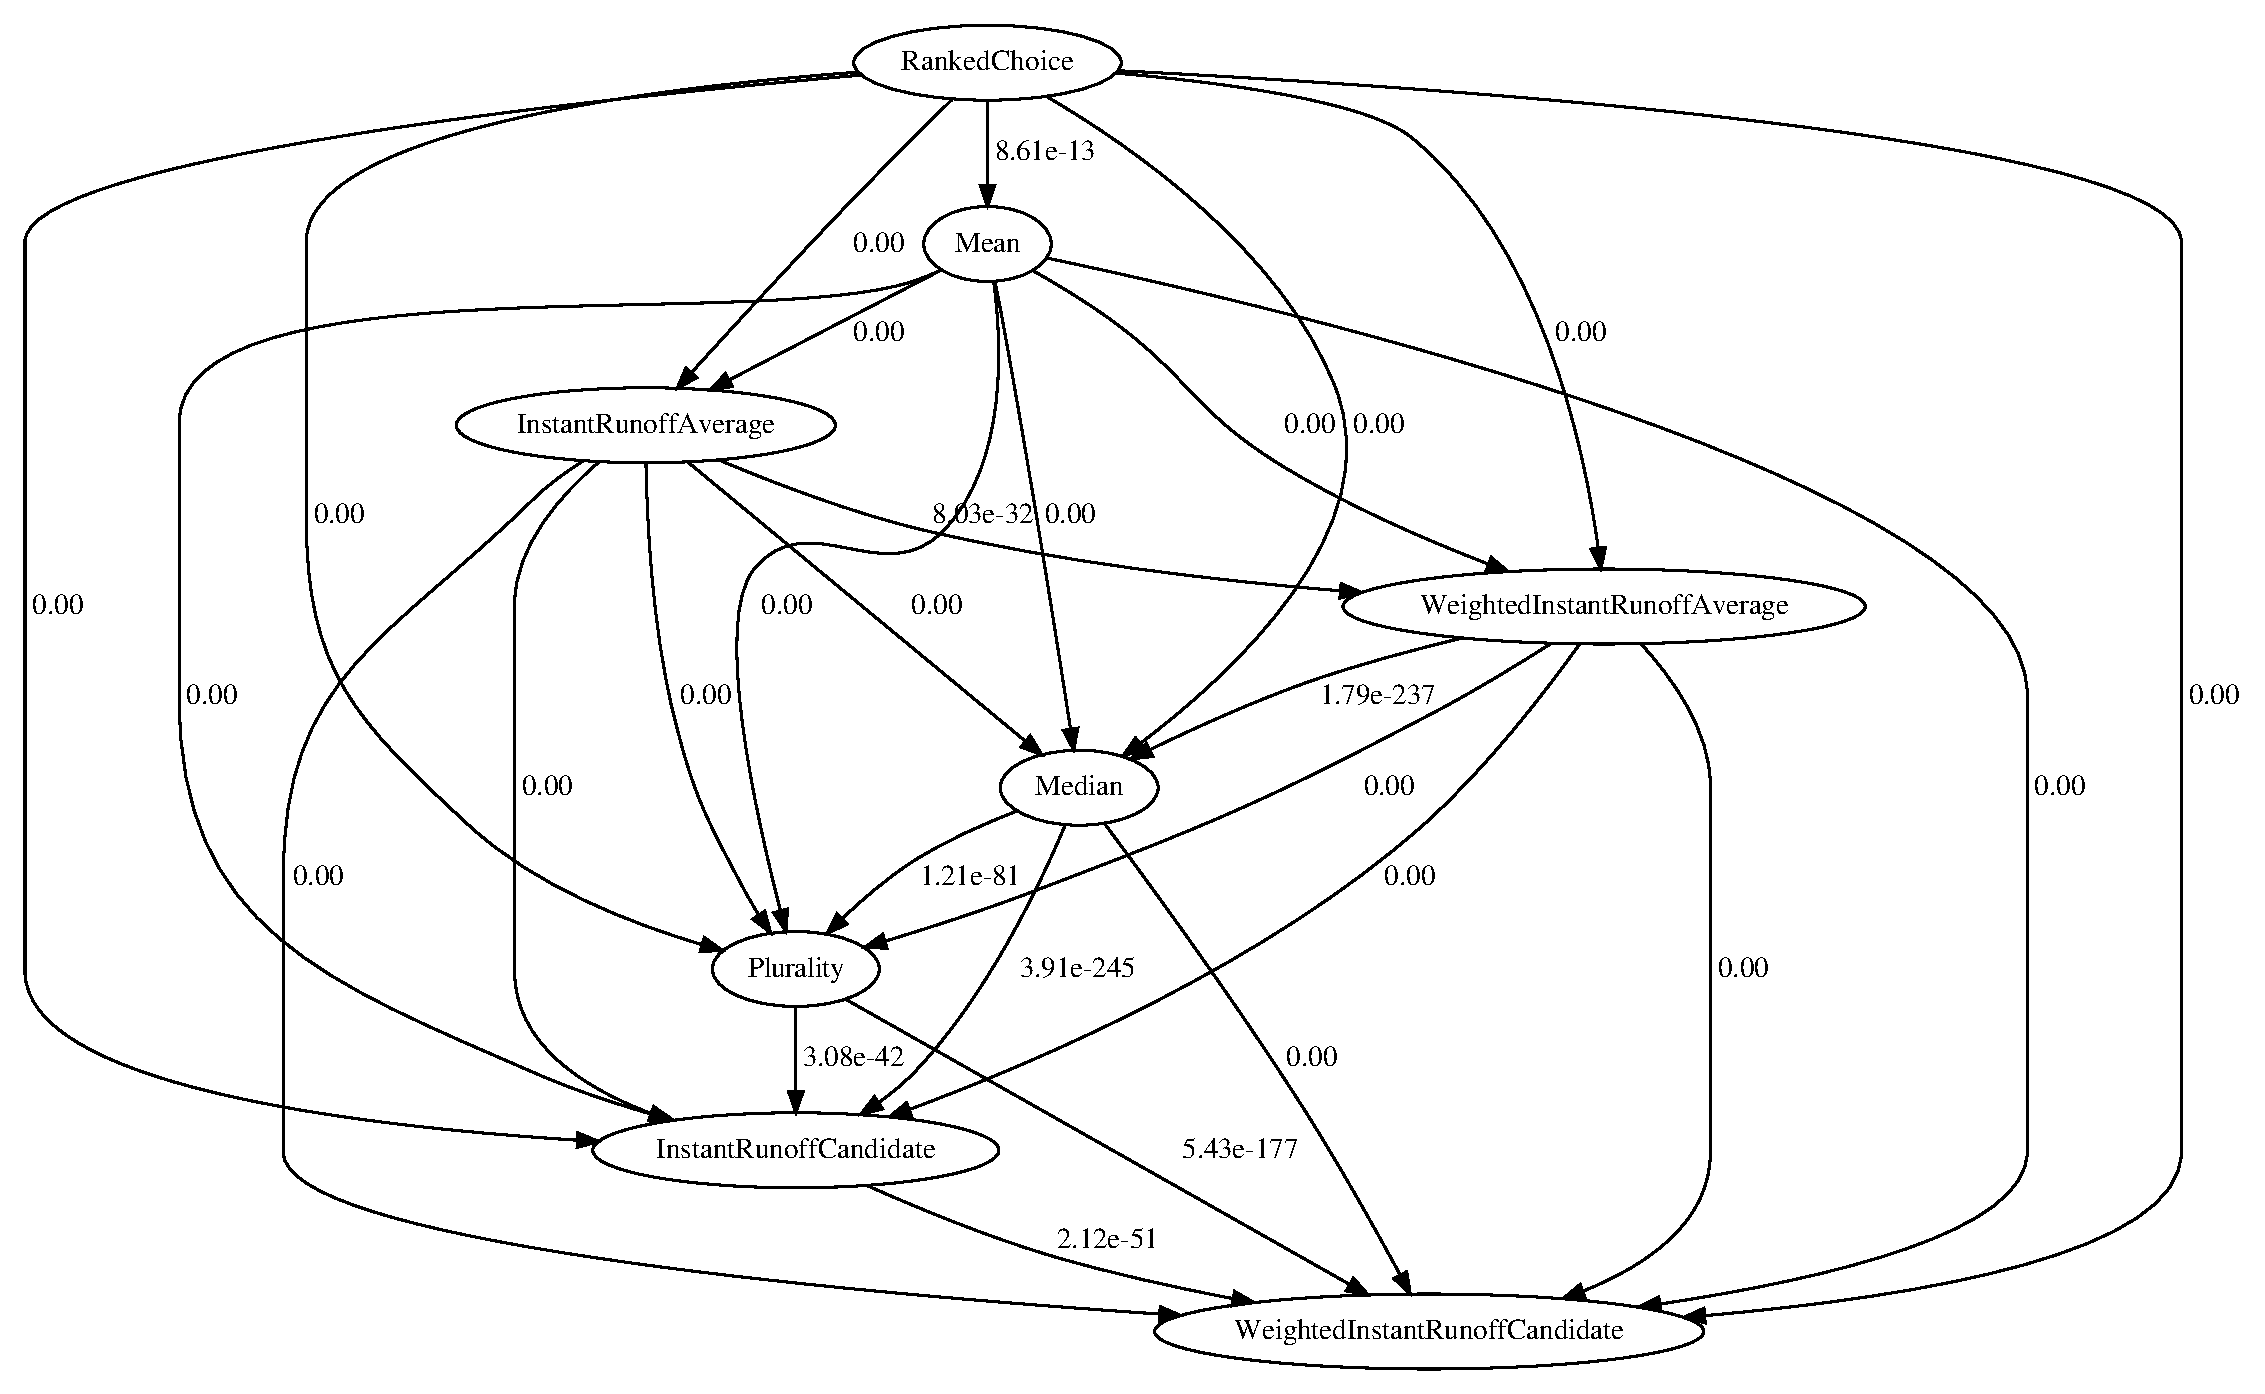
\includegraphics[
        angle=90,
        width=\textwidth,
        height=\dimexpr
        \textheight - 4 % Could also be .9\textheight
        \baselineskip,
        keepaspectratio]
    {./content/figures/voting_mechanisms/all-voting-mechanisms-p-values.gv}
    \caption{The p-values for all voting mechanisms, given the alternative is one
    population is lesser than the other.
    An arrow pointing to another voting mechanism indicates the `from' mechanism beats
    the `to' mechanism.}
    \label{fig:all-voting-mechanisms-p-values}
\end{figure}


\appendixsection{Distributions of Variables}
The distribution of variables for each voting mechanism is displayed as a
KDE graph in \autoref{fig:voting_mechanisms_error_distribution} and
\autoref{fig:voting_mechanisms_estimate_distribution}.

\begin{figure}[!t]
    \centering
    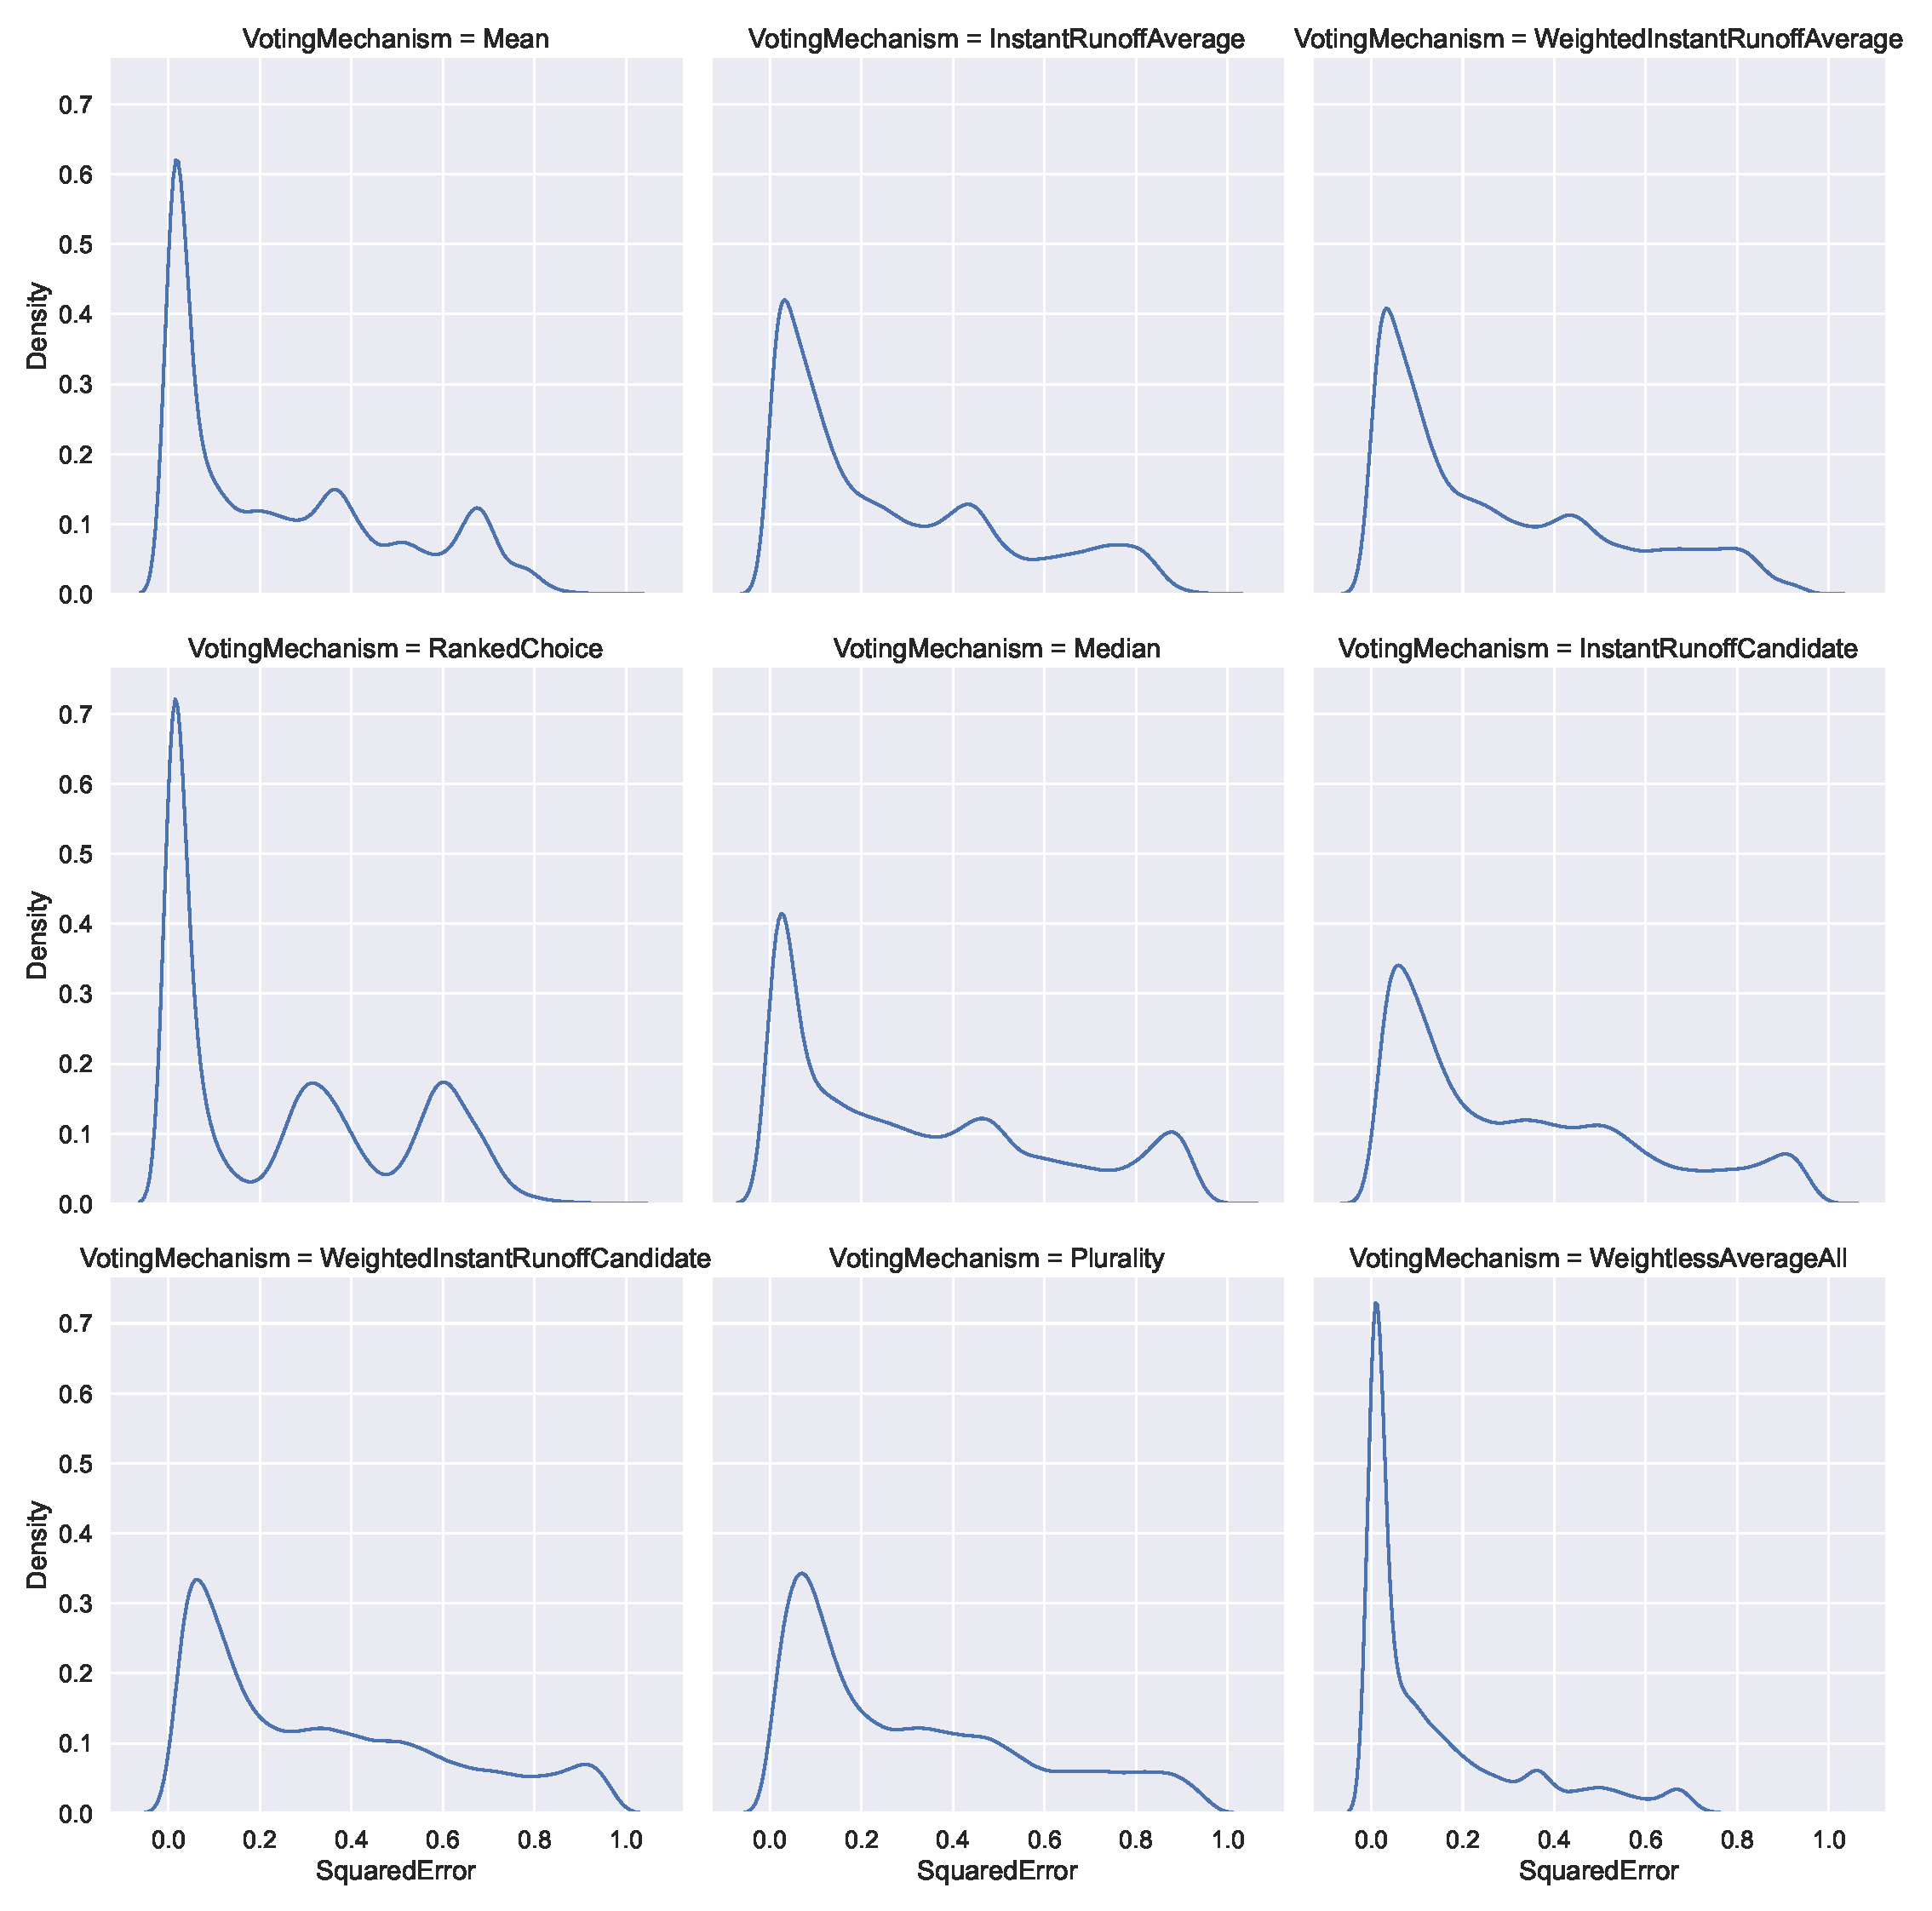
\includegraphics[
        width=\textwidth,
        height=\dimexpr
        \textheight - 2 % Could also be .9\textheight
        \baselineskip,
        keepaspectratio]
    {./content/figures/voting_mechanisms/voting_mechanisms_error_distribution}
    \caption{The distribution of squared error by voting mechanism.}
    \label{fig:voting_mechanisms_error_distribution}
\end{figure}

\begin{figure}[!t]
    \centering
    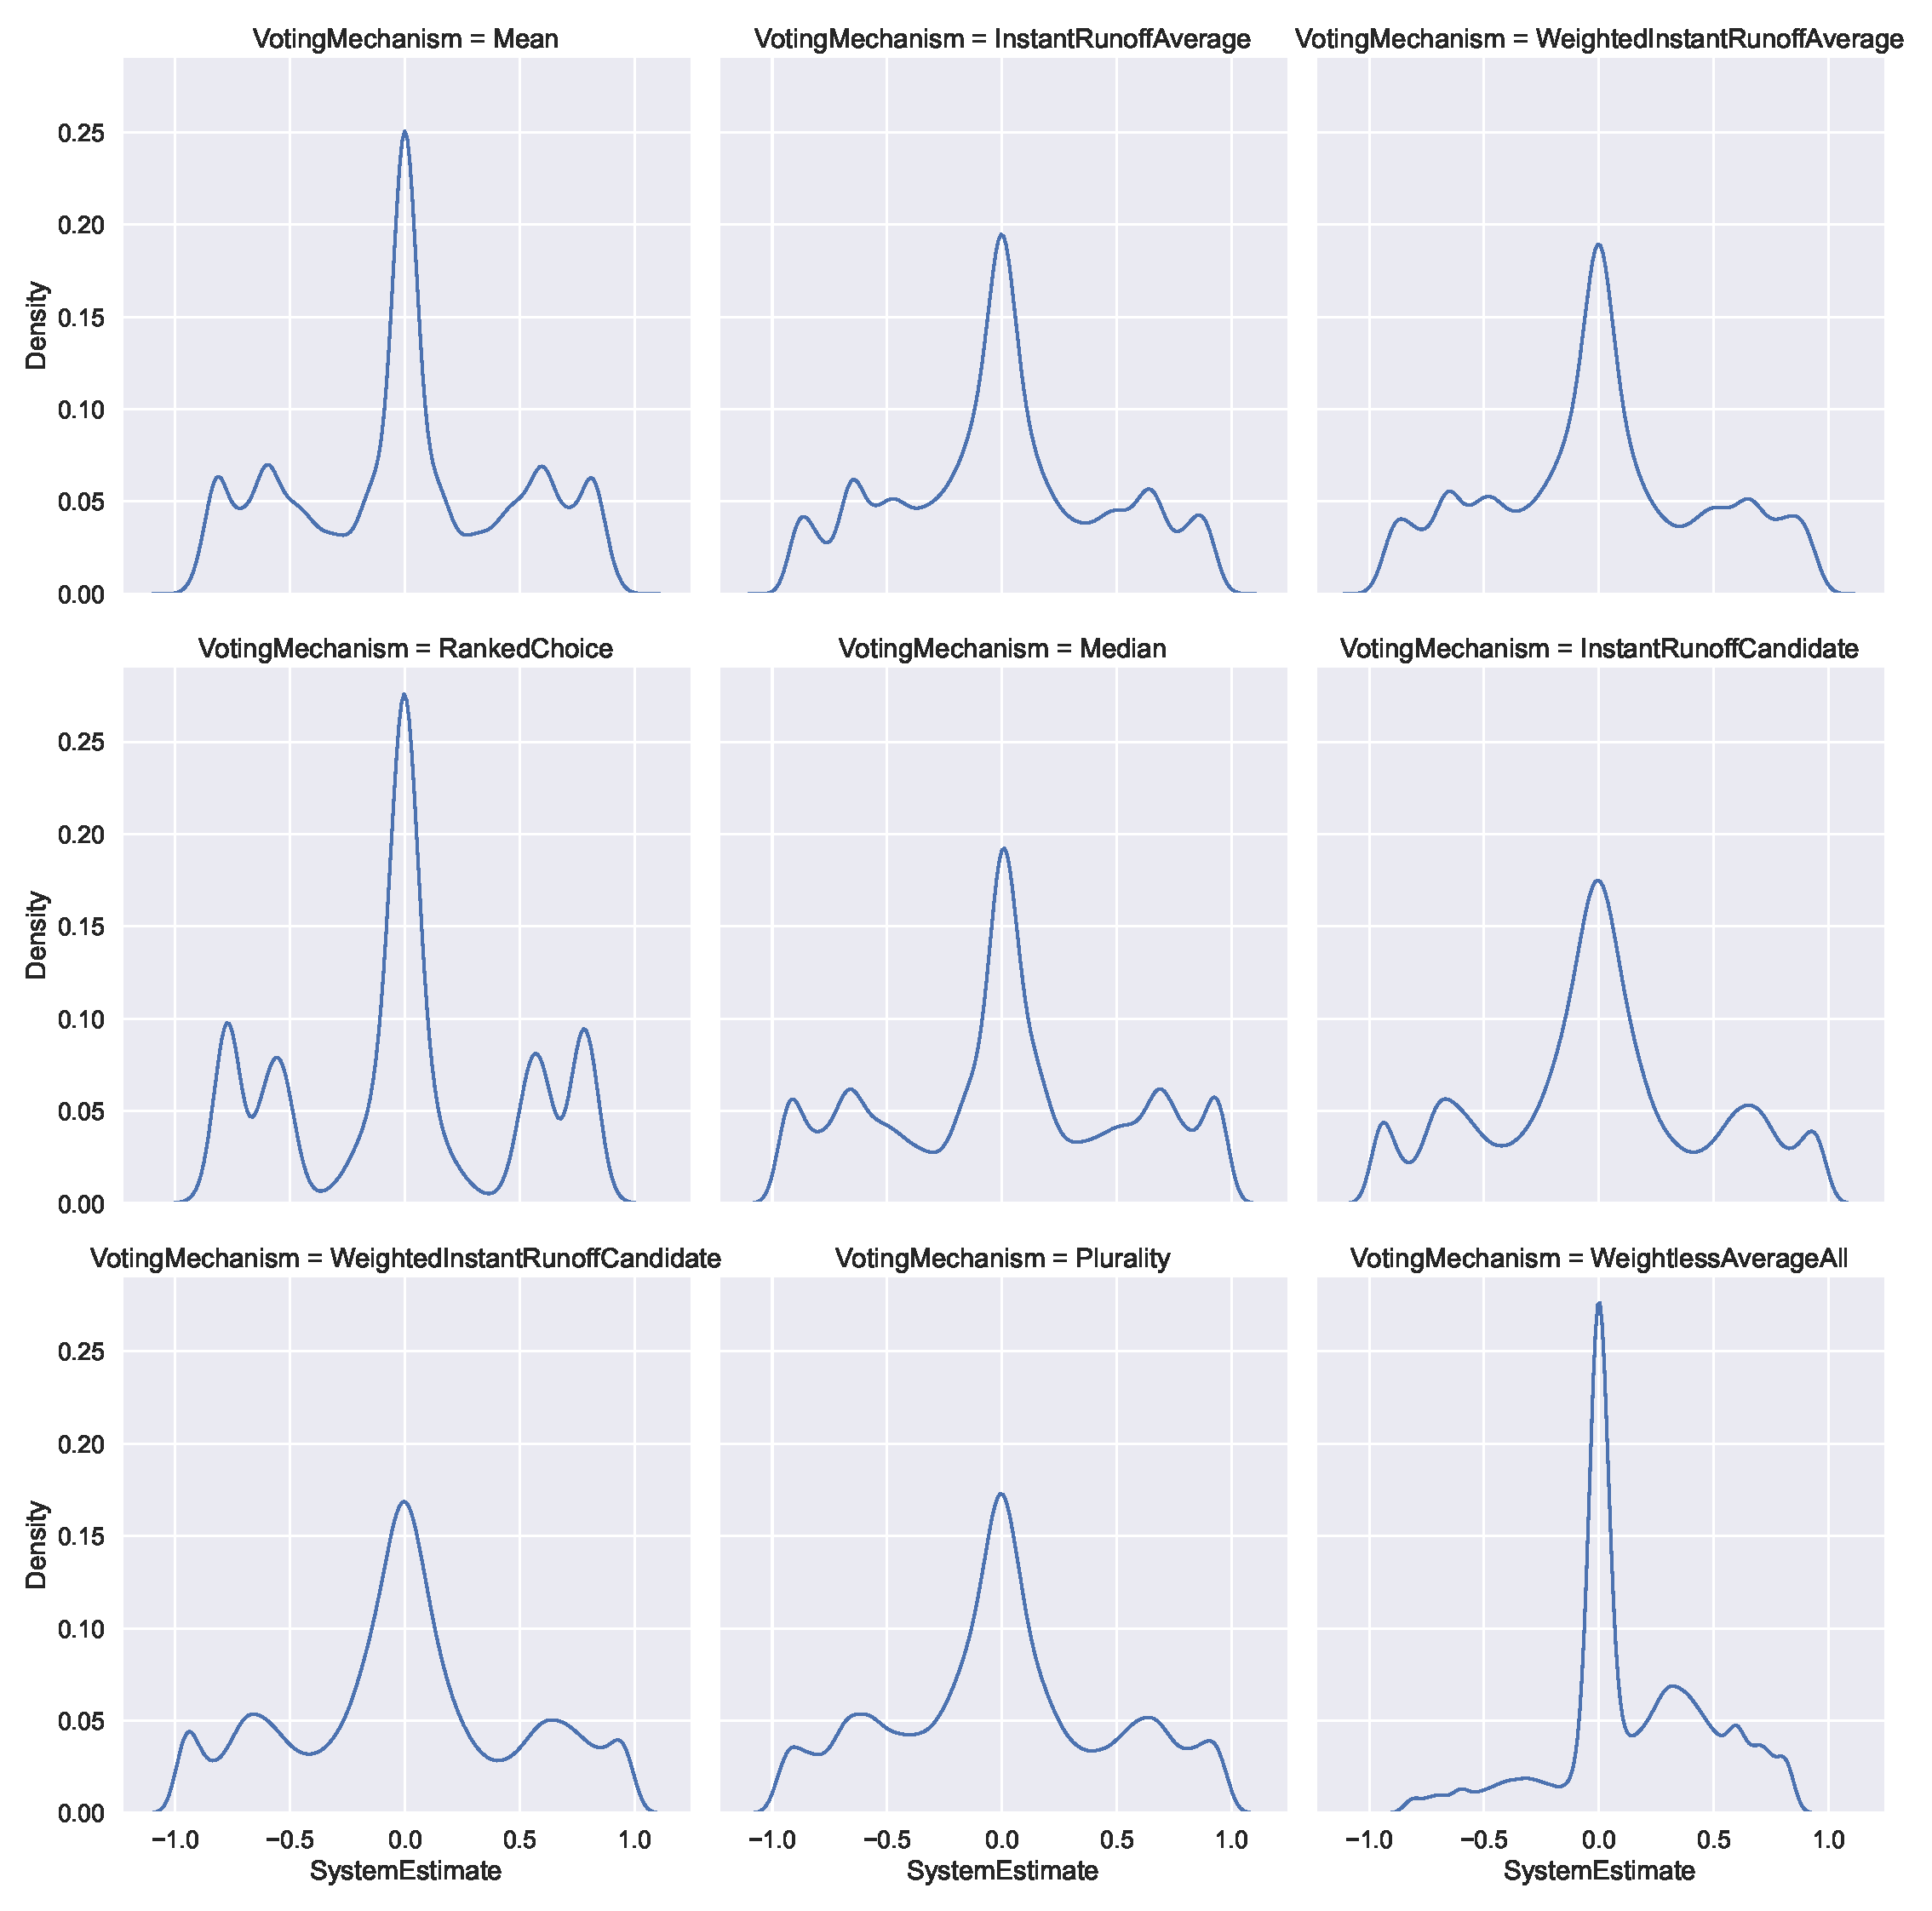
\includegraphics[
        width=\textwidth,
        height=\dimexpr
        \textheight - 2 % Could also be .9\textheight
        \baselineskip,
        keepaspectratio]
    {./content/figures/voting_mechanisms/voting_mechanisms_estimate_distribution}
    \caption{The distribution of system estimate by voting mechanism.}
    \label{fig:voting_mechanisms_estimate_distribution}
\end{figure}

\appendix{Visualizations}\label{chap:visualizations}
\autoref{fig:expected_even_distribution_squared_error} displays the expected look of
a boxen plot when the estimate distribution is uniform, while
\autoref{fig:expected_gaussian_distribution_squared_error} shows the expected look
when the estimate distribution is normal or Gaussian.

\begin{figure}[htbp]
    \centering
    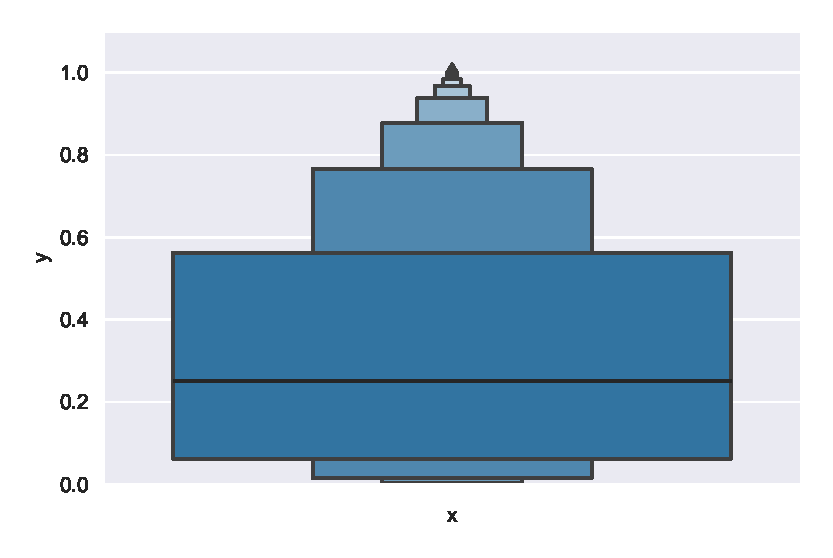
\includegraphics[scale=0.5]
    {./content/figures/expected_even_distribution_squared_error}
    \caption{Expected squared error distribution given a uniform distribution
    of estimates.}
    \label{fig:expected_even_distribution_squared_error}
\end{figure}

\begin{figure}[htbp]
    \centering
    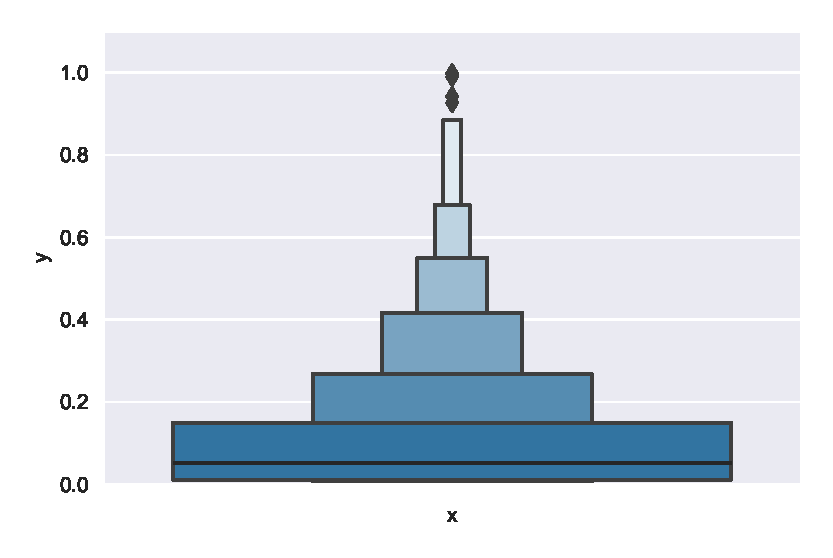
\includegraphics[scale=0.5]
    {./content/figures/expected_gaussian_distribution_squared_error}
    \caption{Expected squared error distribution given a gaussian distribution
    of estimates.}
    \label{fig:expected_gaussian_distribution_squared_error}
\end{figure}
